%%%%%%%%%%%%%%%%%%%%%%%%%%%%%%%%%%%%%%%%%%%%%%%%%%%%%%%%%%%%%%%%%%%%
%% I, the copyright holder of this work, release this work into the
%% public domain. This applies worldwide. In some countries this may
%% not be legally possible; if so: I grant anyone the right to use
%% this work for any purpose, without any conditions, unless such
%% conditions are required by law.
%%%%%%%%%%%%%%%%%%%%%%%%%%%%%%%%%%%%%%%%%%%%%%%%%%%%%%%%%%%%%%%%%%%%

\documentclass{beamer}
\usetheme[faculty=ped]{fibeamer}
\usepackage[utf8]{inputenc}
\usepackage[magyar]{babel}        %% typeset as follows:


\title{Ingerlési protokollok} %% that will be typeset on the
\subtitle{impulzus, ramp, szinuszos, zap protokollok és ismétlések, illetve kombinációk vizsgálata} %% title page.
\author{}
%% These additional packages are used within the document:
\usepackage{ragged2e}  % `\justifying` text
\setbeamercovered{transparent}
\usepackage{booktabs}  % Tables
\usepackage{tabularx}
\usepackage{tikz}      % Diagrams
\usetikzlibrary{calc, shapes, backgrounds}
\usepackage{amsmath, amssymb}
\usepackage{url}       % `\url`s
\usepackage{listings}  % Code listings
\frenchspacing

\begin{document}
  \frame{\maketitle}

  \AtBeginSection[]{% Print an outline at the beginning of sections
	\begin{frame}<beamer>
	\frametitle{Szekció \thesection.}
	\tableofcontents[currentsection]
\end{frame}}

\begin{darkframes}
	\begin{frame}{Áttekintés}
		\tableofcontents
	\end{frame}
	
	\section{Protokollok információtartalma}
	
	\begin{frame}{Vizsgált protokollok beállításai}
	\textit{Stick and Ball} modellt használtunk $\sigma_w = 7\left[mV\right]$ szórású fehér zaj mellett és mind a három (Ra, cm, gpas) passzív paramétert becsültük. \\
	Rögzítettük a mérési időt minden protokollnál $t=500\left[ms\right]$-ra
		\begin{itemize}
			\item \alert{Impulzus (steps)}: $\left(3, 5, 10, 15, 50, 100, 200, 400\right) \left[ms\right]$ ideig $0.5\left[nA\right]$
			\item \alert{Szinusz (zap)}: $\left(1, 2, 3, 4, 5, 10, 25, 50, 75, 150\right) \left[Hz\right]$ + igazi zap $0.2\left[nA\right]$ amplitúdóval
			\item \alert{Rámpa}: $\left(0-0.4\right)\left[nA\right]$ emelkedik $400\left[ms\right]$ alatt
		\end{itemize}
	Egyes protokoll információtartalmát a \textit{szélesség} mennyiségekkel jellemeztük: \\
	\alert{broadness}: 100$\%$ esetén a poszterior olyan éles mint a prior (nem gyűjtöttünk információt)
	\end{frame}
	
	\begin{frame}
		\begin{center}
			\Large \alert{Rámpa}
		\end{center}
	\end{frame}
	
	\begin{frame}
		  \begin{columns}[T]
			\begin{column}{.5\textwidth}
				\begin{figure}
					\centering
					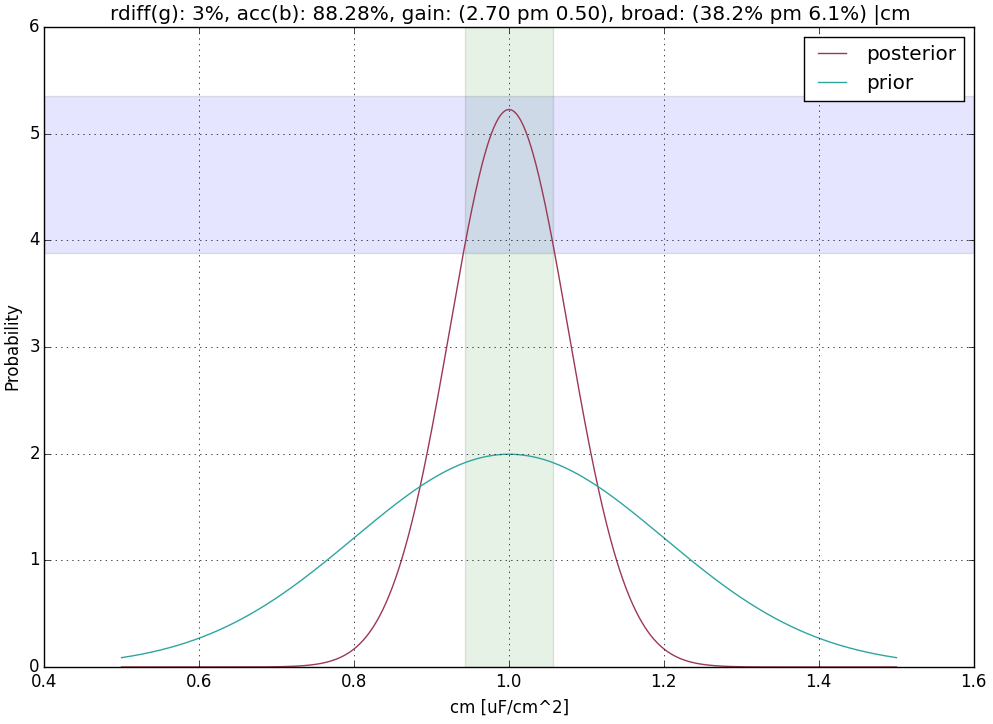
\includegraphics[width=\textwidth]{ramp/illustration_cm.png}
				\end{figure}
				\begin{figure}
					\centering
					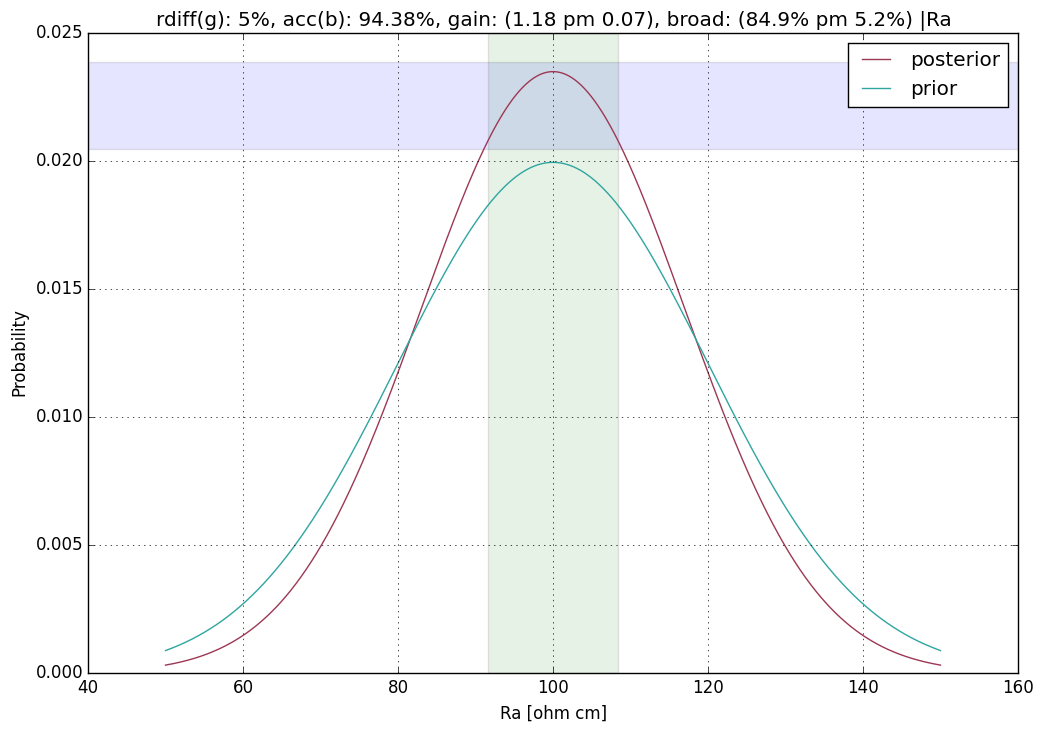
\includegraphics[width=\textwidth]{ramp/illustration_Ra.png}
				\end{figure}
				
			\end{column}
			\begin{column}{.5\textwidth}
				\begin{figure}
					\centering
					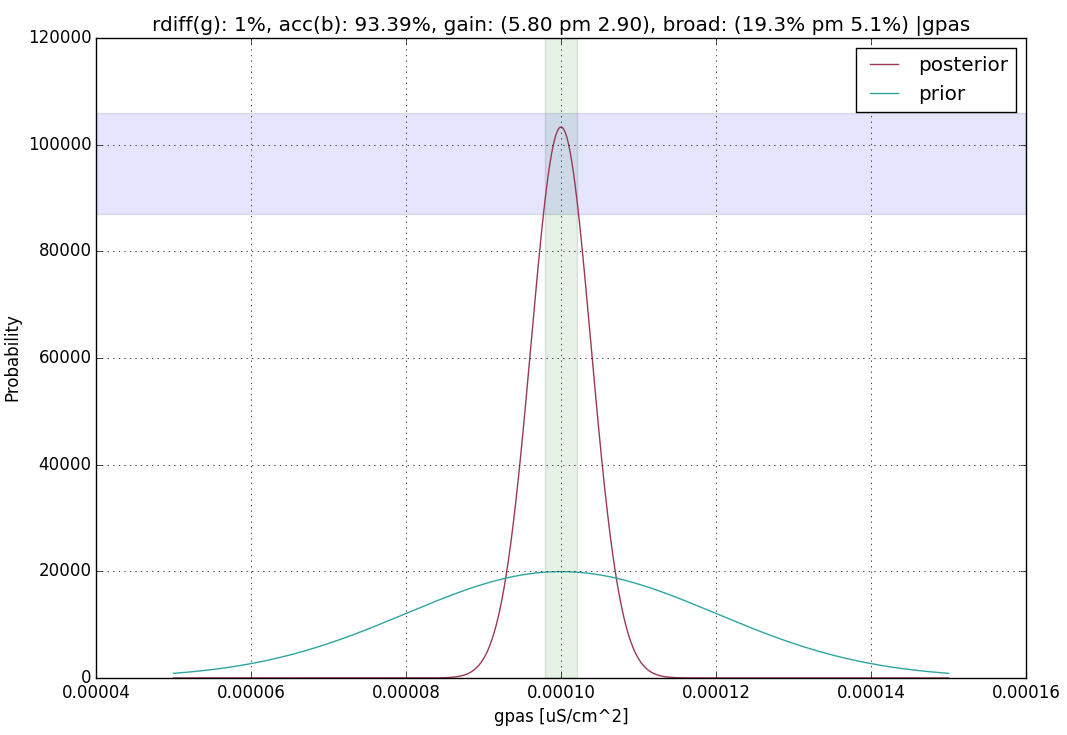
\includegraphics[width=\textwidth]{ramp/illustration_gpas.png}
				\end{figure}

				Ramp protokoll eredményei: 
				\begin{itemize}
					\item Ra szélesség: 84.9$\%$
					\item cm szélesség: 38.2$\%$
					\item gpas szélesség: 19.3$\%$
				\end{itemize}
				
			\end{column}
		\end{columns}
	\end{frame}

\begin{frame}
\begin{center}
	\Large \alert{Impulzusok}
\end{center}
\end{frame}
	\begin{frame}{Impulzus eredmények}
		\begin{figure}
			\centering
			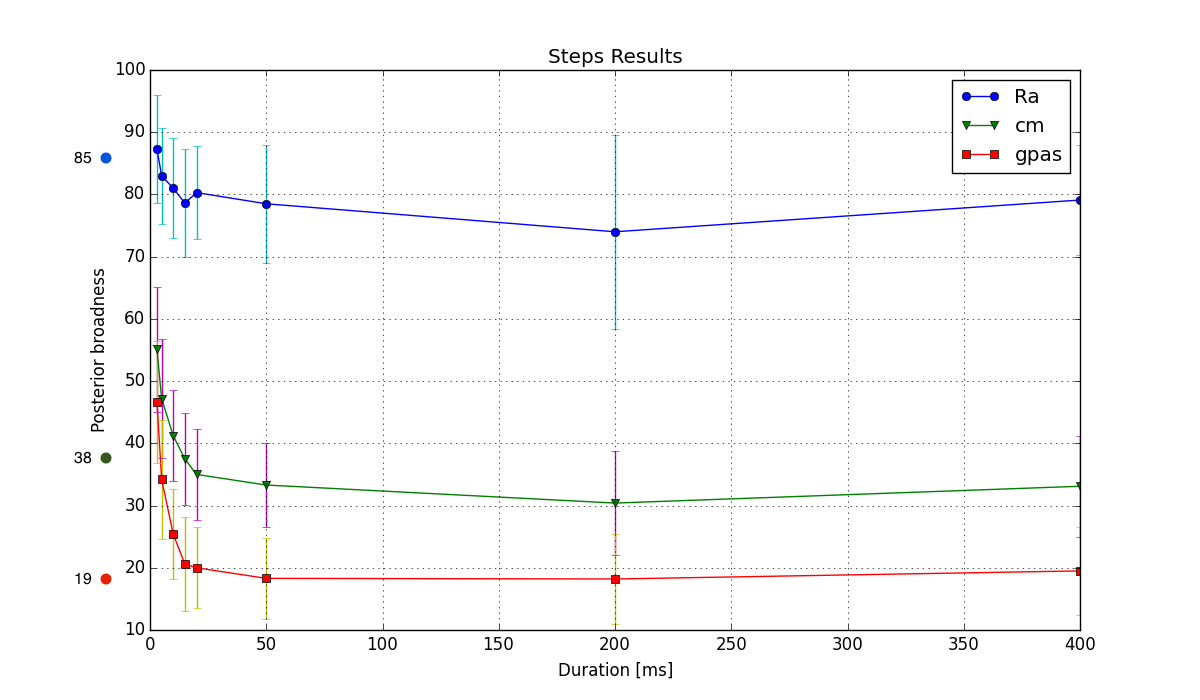
\includegraphics[width=\textwidth]{steps/steps_broadness.png}
		\end{figure}
	\end{frame}

\begin{frame}
\begin{center}
	\Large \alert{Szinuszok}
\end{center}
\end{frame}

	\begin{frame}{Szinuszos eredmények}
	\begin{figure}
		\centering
		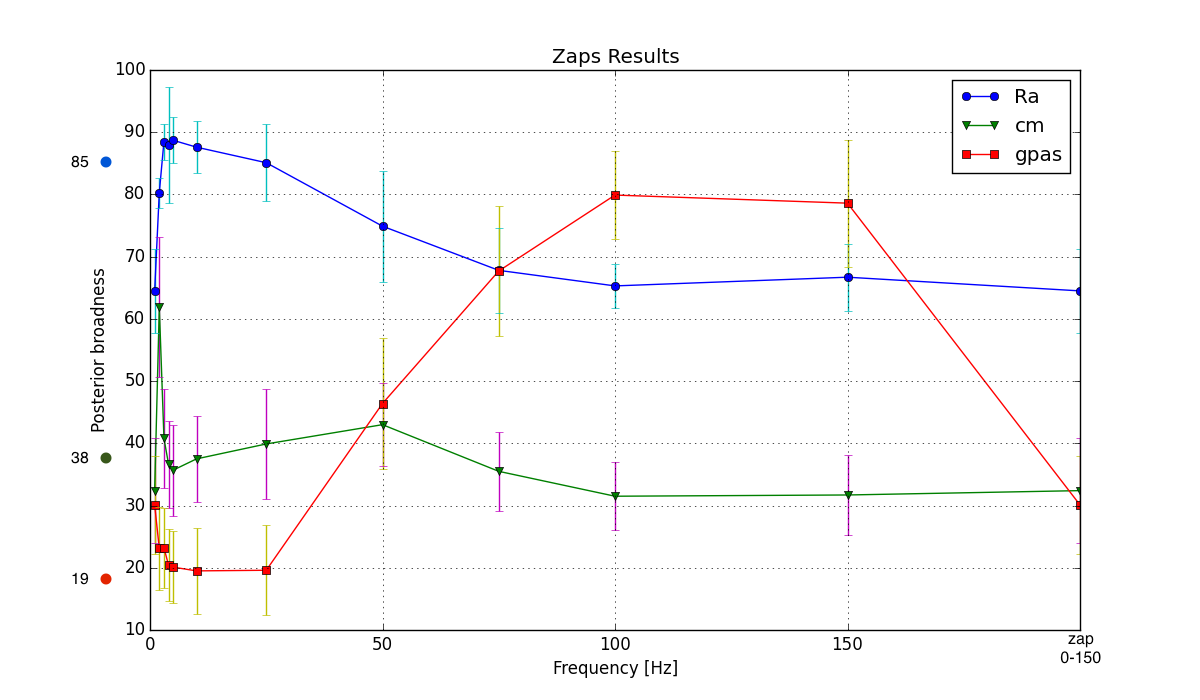
\includegraphics[width=\textwidth]{steps/zaps_broadness.png}
	\end{figure}
	\end{frame}

\section{Ismétlések és kombinációk vizsgálata}

\begin{frame}{Vizsgálat menete}
\begin{itemize}
	\item<1-> 6 db protokollt vizsgáltunk, 3db impulzus és 3db szinuszosat:
	\begin{itemize}
		\item<1-> Impulzus: $\left(3, 20, 200\right)\left[ms\right]$
		\item<1-> Szinusz: $\left(1, 10, 100\right)\left[Hz\right]$
	\end{itemize}
	\item<2-> Mindegyik protokollhoz megcsináltuk a becslést 10 különböző kiindulási paraméterre.
	\item<3-> Mind a 10 paraméterhez csináltunk 30db ismétlést (csak a zaj változott).
	\item<4-> Kiindulási paraméterek hatása az inferenciára?
	\item<5-> Impulzus és Szinusz protokollokat külön vizsgáltuk.
	\item<6-> Egyes protokollok 30 db ismétlésből származó eredményeinek szorzata, vagy a 3 különböző protokoll kombinálása a jobb?
	
\end{itemize}


\end{frame}

\begin{frame}
	\begin{center}
		\Large \alert{Impulzusok}
	\end{center}
\end{frame}


\begin{frame}
\begin{columns}[T]
	\begin{column}{.5\textwidth}
		\begin{figure}
			\centering
			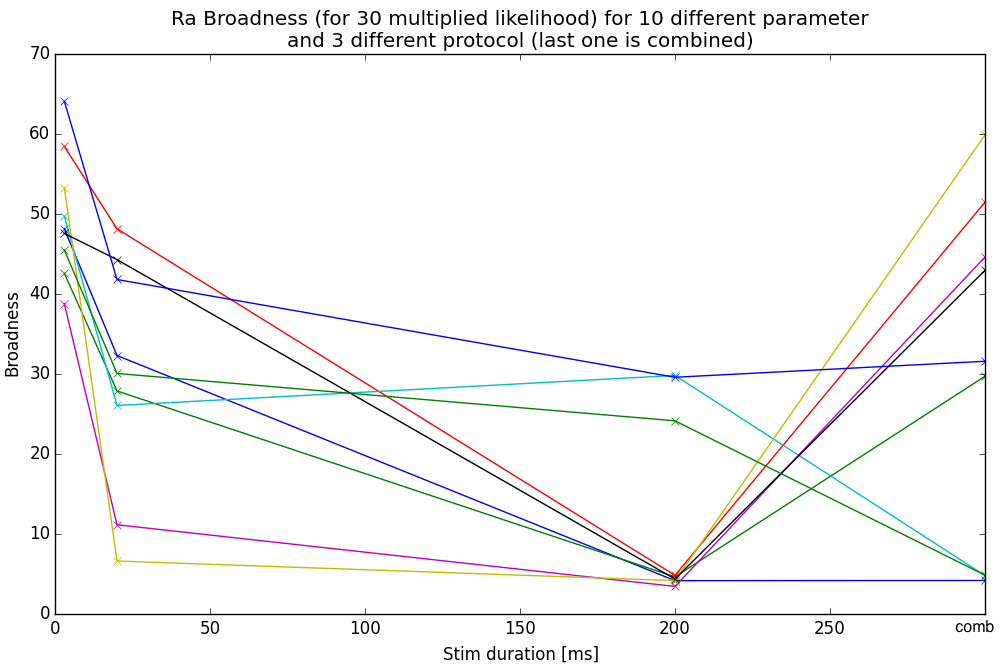
\includegraphics[width=\textwidth]{comb/steps/Ra_brod.png}
		\end{figure}
		\begin{figure}
			\centering
			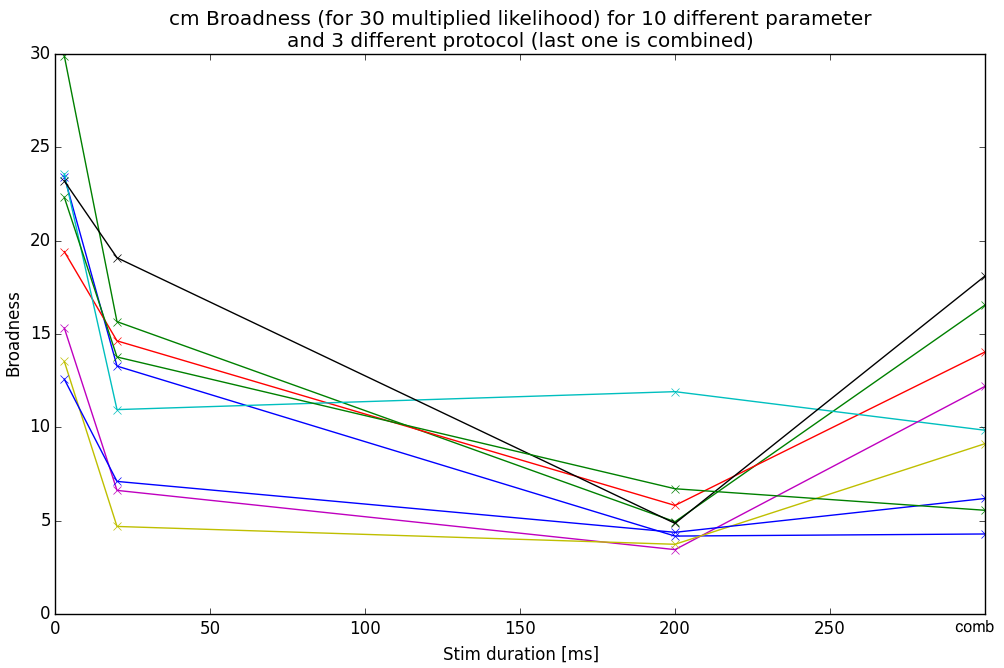
\includegraphics[width=\textwidth]{comb/steps/cm_brod.png}
		\end{figure}
		
	\end{column}
	\begin{column}{.5\textwidth}
		\begin{figure}
			\centering
			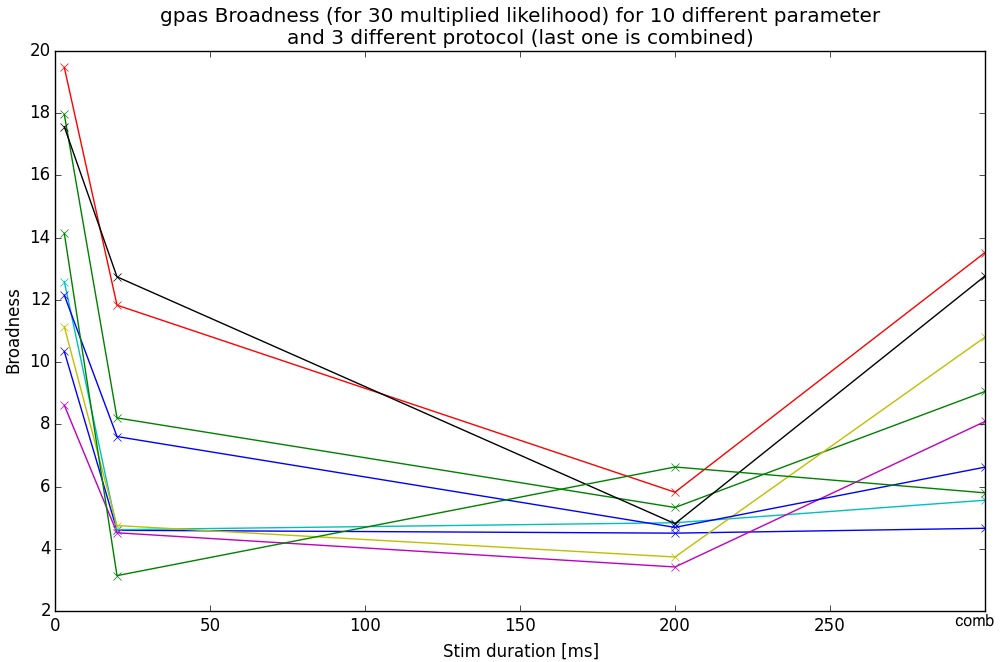
\includegraphics[width=\textwidth]{comb/steps/gpas_brod.png}
		\end{figure}
		\alert{Step broadness eredmények}\\
		30 különböző zajmegvalósulás eredményeit szoroztuk egyes paraméterekre és vizsgáltunk 10 különböző kiindulási paramétert.\\
		\alert{Utolsó pont a kombinált!}
		
	\end{column}
\end{columns}
\end{frame}


\begin{frame}{Multiplikált/kombinált impulzus eredmények}
\begin{figure}
	\centering
	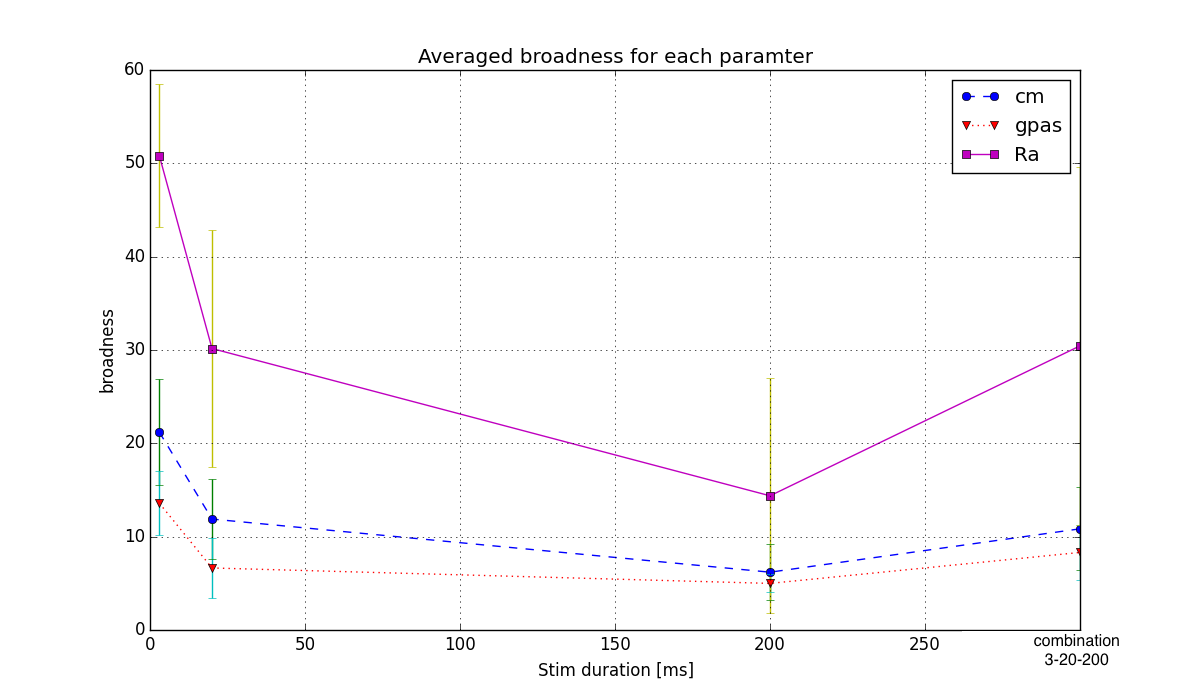
\includegraphics[width=\textwidth]{comb/steps/avrg_broadness.png}
\end{figure}
\end{frame}



\begin{frame}
\begin{center}
	\Large \alert{Szinuszok}
\end{center}
\end{frame}

\begin{frame}
\begin{columns}[T]
\begin{column}{.5\textwidth}
	\begin{figure}
		\centering
		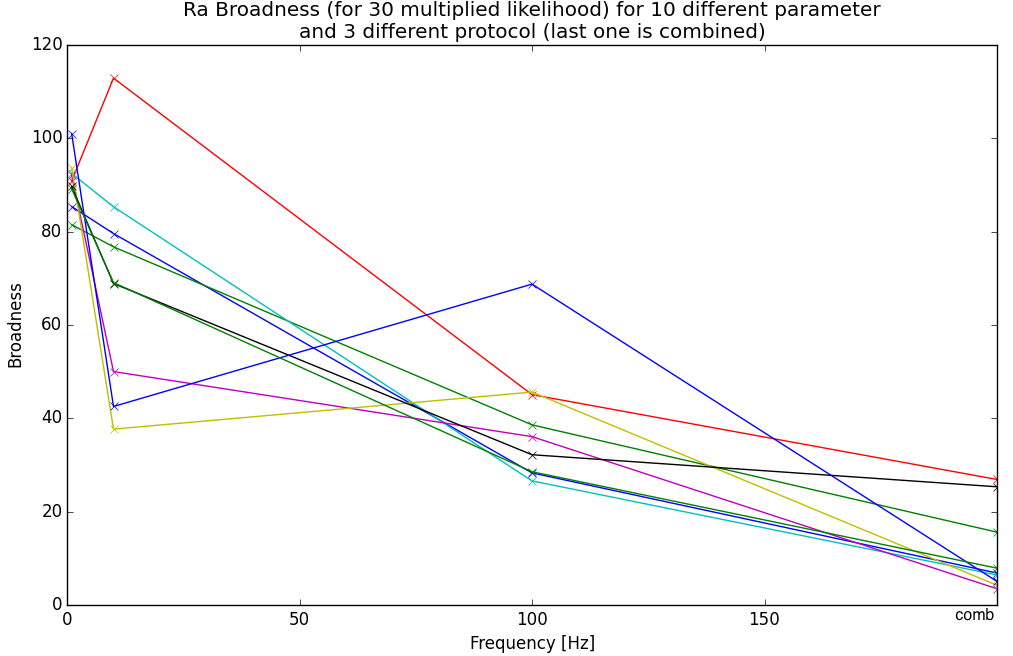
\includegraphics[width=\textwidth]{comb/zaps/Ra_brod.png}
	\end{figure}
	\begin{figure}
		\centering
		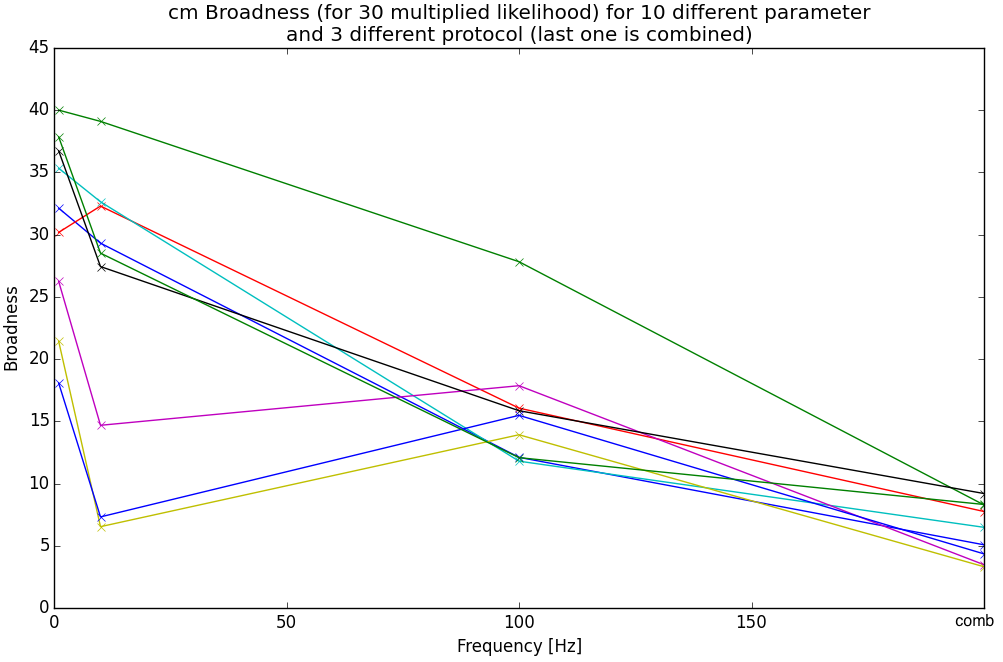
\includegraphics[width=\textwidth]{comb/zaps/cm_brod.png}
	\end{figure}
	
\end{column}
\begin{column}{.5\textwidth}
	\begin{figure}
		\centering
		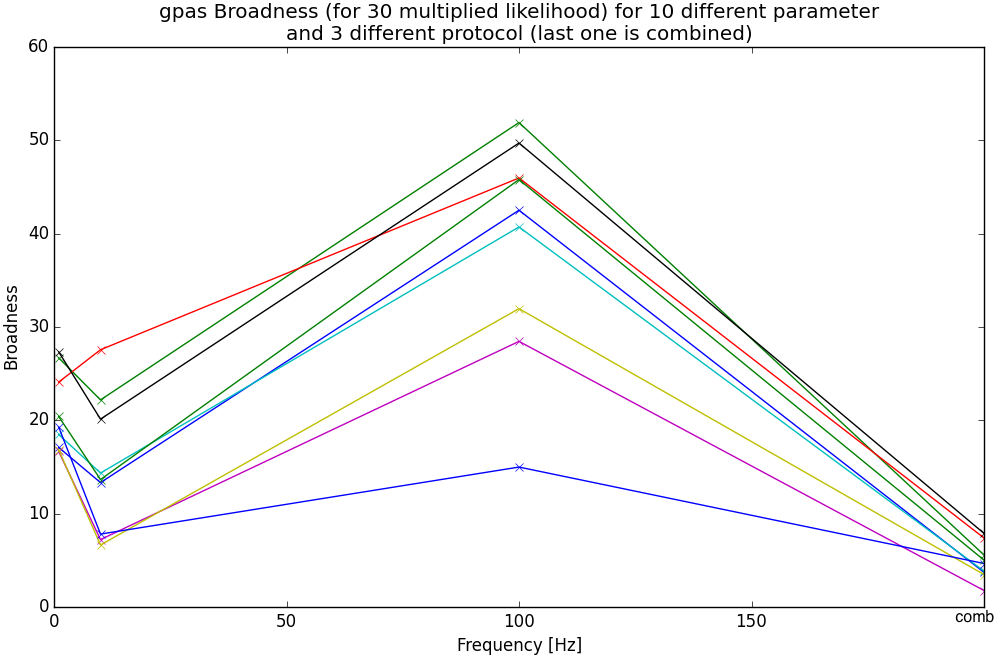
\includegraphics[width=\textwidth]{comb/zaps/gpas_brod.png}
	\end{figure}
	\alert{Szinusz broadness eredmények}\\
	30 különböző zajmegvalósulás eredményeit szoroztuk egyes paraméterekre és vizsgáltunk 10 különböző kiindulási paramétert. \\
	\alert{Utolsó pont a kombinált!}
\end{column}
\end{columns}
\end{frame}


\begin{frame}{Multiplikált/kombinált Szinusz eredmények}
\begin{figure}
\centering
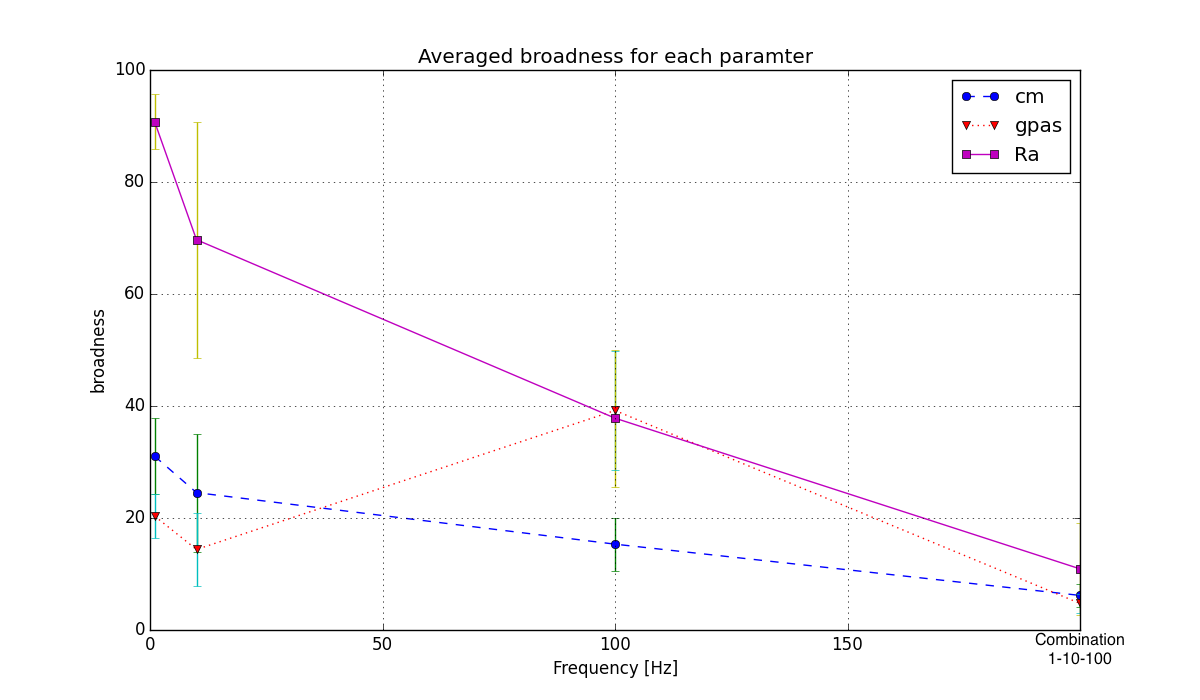
\includegraphics[width=\textwidth]{comb/zaps/avrg_broadness.png}
\end{figure}
\end{frame}

\end{darkframes}


\end{document}
